\renewcommand{\FileName}{assoc}
\subsection{Nominal factors}
\begin{frame}[fragile]
  \frametitle{Testing Association in Two-Way Tables}
  \begin{block}{\large\bfseries Typical analysis: Nominal factors}
  \end{block}
      \begin{itemize}
	  \item Pearson $\chisq$ (or LR $\chisq$)--- when most expected
	  frequencies $\ge 5$.

\begin{listing}[frame=single]
proc freq;
   weight count;        \sascomment{/* if in frequency form */}
   table factor * response / \sasemph{chisq}; 
\end{listing}

	  \item Exact tests--- small tables, small sample sizes (e.g., Fisher's)

\begin{listing}[frame=single]
proc freq;
   weight count;        \sascomment{/* if in frequency form */}
   table factor * response / \sasemph{chisq};
   \sasemph{exact pchi;}
\end{listing}
	  \end{itemize}
\end{frame}

\begin{frame}[fragile]
  \frametitle{Example: Cholesterol diet and heart disease}
Is there a relation between Hi/Lo cholesterol diet and heart disease?
\vspace{2ex}

\begin{Input}[fontsize=\footnotesize,label=\fbox{\texttt{fat.sas}},baselinestretch=0.8]
title 'Cholesterol diet and heart disease';
data fat;
   input diet $ disease $ count;
datalines;
LoChol  No   6
LoChol  Yes  2
HiChol  No   4
HiChol  Yes 11
;

proc freq data=fat;
  weight count;
  tables diet * disease / chisq nopercent nocol;
  \sasemph{exact pchi};
\end{Input}
\end{frame}

\begin{frame}[fragile]
Standard output:
\begin{Output}[fontsize=\footnotesize,gobble=7,baselinestretch=.7]
                           Table of diet by disease

                     diet      disease

                     Frequency|
                     Row Pct  |No      |Yes     |  Total
                     ---------+--------+--------+
                     HiChol   |      4 |     11 |     15
                              |  26.67 |  73.33 |
                     ---------+--------+--------+
                     LoChol   |      6 |      2 |      8
                              |  75.00 |  25.00 |
                     ---------+--------+--------+
                     Total          10       13       23


                   Statistics for Table of diet by disease

            Statistic                     DF       Value      Prob
            ------------------------------------------------------
            Chi-Square                     1      4.9597    0.0259
            Likelihood Ratio Chi-Square    1      5.0975    0.0240
            Continuity Adj. Chi-Square     1      3.1879    \sasemph{0.0742}

         \sasemph{WARNING}: 50% of the cells have expected counts less than 5. 
                  (Asymptotic) Chi-Square may not be a valid test.
\end{Output}
\begin{itemize*}
  \item The Pearson and LR $\chisq$ tests are \emph{not valid}--- sample size too small
  \item The conservative continuity-adjusted test fails significance
\end{itemize*}
\end{frame}

\begin{frame}[fragile]
\begin{itemize*}
  \item Exact tests are \emph{valid} and significant.
\end{itemize*}
Exact test output:
\begin{Output}[fontsize=\footnotesize,gobble=7,baselinestretch=.8]
            		   Pearson Chi-Square Test
        		  ----------------------------------
        		  Chi-Square                  4.9597
        		  DF                               1
        		  Asymptotic Pr >  ChiSq      0.0259
        		  Exact      Pr >= ChiSq      0.0393


                		 Fisher's Exact Test
        		  ----------------------------------
        		  Cell (1,1) Frequency (F)         4
        		  Left-sided Pr <= F          0.0367
        		  Right-sided Pr >= F         0.9967

        		  Table Probability (P)       0.0334
        		  Two-sided Pr <= P           \sasemph{0.0393}
\end{Output}

\end{frame}

\begin{frame}[fragile]
  \frametitle{Preview: Visualizing association in 2 $\times$ 2 tables}
 \begin{minipage}[c]{.5\linewidth}
  \centering
  \includegraphics[width=.9\linewidth,clip]{fig/fat2}
 \end{minipage}%
 \begin{minipage}[c]{.5\linewidth}
   \begin{itemize}
    \item Fourfold display: area $\sim$ frequency
    \item Color: \blue{blue} ($+$), \red{red}($-$)
    \item Confidence bands: significance of odds ratio
    \item Interp: Hi cholesterol $\rightarrow$ Heart disease
   \end{itemize}
 \end{minipage}
\vspace{1ex}
\begin{listing}[frame=single]
%ffold(data=fat, var=diet disease);
\end{listing}

\end{frame}

\subsection{Ordinal factors and Stratified analyses}
\begin{frame}[fragile]
  \frametitle{Ordinal factors and Stratified analyses}

  \begin{block}{\large\bfseries More powerful CMH tests}
      \begin{itemize*}
	  \item When either the row (factor) or column (response) levels are
	  \alert{ordered}, more specific (CMH = Cochran - Mantel - Haentzel) tests
	  which take order into account have greater power to detect ordered
	  relations.
\begin{listing}[frame=single]
proc freq;
   weight count;
   table factor * response / chisq \sasemph{cmh}; 
\end{listing}
	  \end{itemize*}
  \end{block}
  \begin{block}{\large\bfseries Control for other background variables} 
      \begin{itemize*}
	    \item Stratified analysis tests the association between a main
		factor and response \emph{within}  levels of the control
		variable(s)
		\item Can also test for homogeneous association across strata
\begin{listing}[frame=single]
proc freq;
   weight count;
   table \sasemph{strata} * factor * response / chisq \sasemph{cmh}; 
\end{listing}
	  \end{itemize*}
  \end{block}
\end{frame}

% slide template
\begin{frame}[fragile]
  \frametitle{Example: Arthritis treatment}
  Data on treatment for rheumatoid arthritis \citep{KochEdwards:88}
  \begin{itemize}
	\item {\large\bfseries Ordinal response}: none, some, or marked improvement
	\item {\large\bfseries Factor}:  active treatment vs.\ placebo
	\item{\large\bfseries Strata}:  Sex
  \end{itemize}
\begin{listing}
                      |         Outcome
   ---------+---------+--------------------------+
   Treatment|  Sex    |None    |Some    |Marked  |  Total
   ---------+---------+--------+--------+--------+
   Active   |  Female |      6 |      5 |     16 |     27
            |  Male   |      7 |      2 |      5 |     14
   ---------+---------+--------+--------+--------+
   Placebo  |  Female |     19 |      7 |      6 |     32
            |  Male   |     10 |      0 |      1 |     11
   ---------+---------+--------+--------+--------+
   Total                    42       14       28       84
\end{listing}
\end{frame}

\begin{frame}[fragile]
{\bfseries Overall analysis, ignoring sex}:
\begin{Input}[fontsize=\footnotesize,label=\fbox{\texttt{arthfreq.sas} $\cdots$},baselinestretch=0.8]
title 'Arthritis Treatment: PROC FREQ Analysis';
data arth;
   input sex$ treat$ @;
   do improve = 'None  ', 'Some', 'Marked';
      input count @;
      output;
      end;
datalines;
Female  Active    6  5  16
Female  Placebo  19  7   6
Male    Active    7  2   5
Male    Placebo  10  0   1
;
\sascomment{*-- Ignoring sex;}
proc freq \sasemph{order=data};
   weight count;
   tables treat * improve / \sasemph{cmh} chisq nocol nopercent;
   run;
\end{Input}
{\bfseries Notes}:

\begin{itemize*}

  \item \PROC{FREQ} orders character variables alphabetically (i.e., `Marked', `None', `Some') by
   default.  
  \item To treat the IMPROVE variable as
   ordinal, use \alert{\texttt{order=data}} on the \PROC{FREQ}
   statement.

%  \item The \opt{chisq}{FREQ} gives the usual \(\chi^2\) tests
%   (Pearson, Fisher's, etc.).  The \opt{cmh}{FREQ} requests the
%   \IX{Cochran-Mantel-Haenszel tests} for ordinal variables.
\end{itemize*}
\end{frame}

\begin{frame}[fragile]
\bfseries{Overall analysis, ignoring sex}: Results (\texttt{chisq} option)
\begin{Output}[gobble=2]
             STATISTICS FOR TABLE OF TREAT BY IMPROVE

      Statistic                     DF     Value        Prob
      ------------------------------------------------------
      Chi-Square                     2    13.055       0.001
      Likelihood Ratio Chi-Square    2    13.530       0.001
      Mantel-Haenszel Chi-Square     1    12.859       0.000
      Phi Coefficient                      0.394
      Contingency Coefficient              0.367
      Cramer's V                           0.394
\end{Output}
Cochran-Mantel-Haenszel tests: (\texttt{cmh} option)
\begin{Output}[gobble=4]
               SUMMARY STATISTICS FOR TREAT BY IMPROVE
      Cochran-Mantel-Haenszel Statistics (Based on Table Scores)

    Statistic   Alternative Hypothesis    DF       Value      Prob
    --------------------------------------------------------------
       1        Nonzero Correlation        1      12.859     0.000
       2        Row Mean Scores Differ     1      12.859     0.000
       3        General Association        2      12.900     0.002
\end{Output}
\end{frame}

\subsection{CMH tests for ordinal variables}
\begin{frame}
\frametitle{CMH tests for ordinal variables}
Three types of test:
  \begin{block}{\large\bfseries Non-zero correlation} 
	  \begin{itemize*}
	  \item Use when \emph{both} row and column variables are ordinal.
	  \item CMH \(\chi^2 = ( N - 1) r^2\), assigning scores (1, 2, 3, ...)
	  \item most powerful for \emph{linear} association
	  \end{itemize*}
  \end{block}
  \begin{block}{\large\bfseries Row Mean Scores Differ} 
      \begin{itemize*}
	  \item Use when only \emph{column} variable is ordinal
	  \item Analogous to the Kruskal-Wallis non-parametric test (ANOVA on rank scores)
	  \item Ordinal variable must be listed \alert{last} in the \texttt{TABLES} statement
       \end{itemize*}
  \end{block}
  \begin{block}{\large\bfseries General Association} 
      \begin{itemize*}
	  \item Use when \emph{both} row and column variables are nominal.
	  \item Similar to overall Pearson \(\chi^2\) and Likelihood Ratio \(\chi^2\).
       \end{itemize*}
  \end{block}
\end{frame}

\begin{frame}[fragile,t]
  \frametitle{Sample CMH Profiles}
  \boldital{Only general association:}
\begin{listing}
        | b1    | b2    | b3    | b4    | b5    |  Total  Mean
--------+-------+-------+-------+-------+-------+
  a1    |     0 |    15 |    25 |    15 |     0 |     55   3.0
  a2    |     5 |    20 |     5 |    20 |     5 |     55   3.0
  a3    |    20 |     5 |     5 |     5 |    20 |     55   3.0
--------+-------+-------+-------+-------+-------+
Total        25      40      35      40      25      165
\end{listing}
\vspace{2ex}
Output:
\begin{Output}[gobble=4]
      Cochran-Mantel-Haenszel Statistics (Based on Table Scores)

    Statistic   Alternative Hypothesis    DF       Value      Prob
    --------------------------------------------------------------
       1        Nonzero Correlation        1       0.000     1.000
       2        Row Mean Scores Differ     2       0.000     1.000
       3        General Association        8      91.797     \sasemph{0.000}
\end{Output}
\end{frame}

\begin{frame}[fragile,t]
  \frametitle{Sample CMH Profiles}
\boldital{Linear Association:}

\begin{listing}
        | b1    | b2    | b3    | b4    | b5    |  Total   Mean
--------+-------+-------+-------+-------+-------+
  a1    |     2 |     5 |     8 |     8 |     8 |     31   3.48
  a2    |     2 |     8 |     8 |     8 |     5 |     31   3.19
  a3    |     5 |     8 |     8 |     8 |     2 |     31   2.81
  a4    |     8 |     8 |     8 |     5 |     2 |     31   2.52
--------+-------+-------+-------+-------+-------+
Total        17      29      32      29      17      124
\end{listing}
\vspace{2ex}
Output:
\begin{Output}[gobble=4]
      Cochran-Mantel-Haenszel Statistics (Based on Table Scores)

    Statistic   Alternative Hypothesis    DF       Value      Prob
    --------------------------------------------------------------
       1        Nonzero Correlation        1      10.639     \sasemph{0.001}
       2        Row Mean Scores Differ     3      10.676     \sasemph{0.014}
       3        General Association       12      13.400     0.341
\end{Output}
\end{frame}

\begin{frame}
  \frametitle{Sample CMH Profiles}
\boldital{Visualizing Association:} Sieve diagrams

\vspace{2ex}
 \begin{minipage}[b]{.5\linewidth}
  \centering
  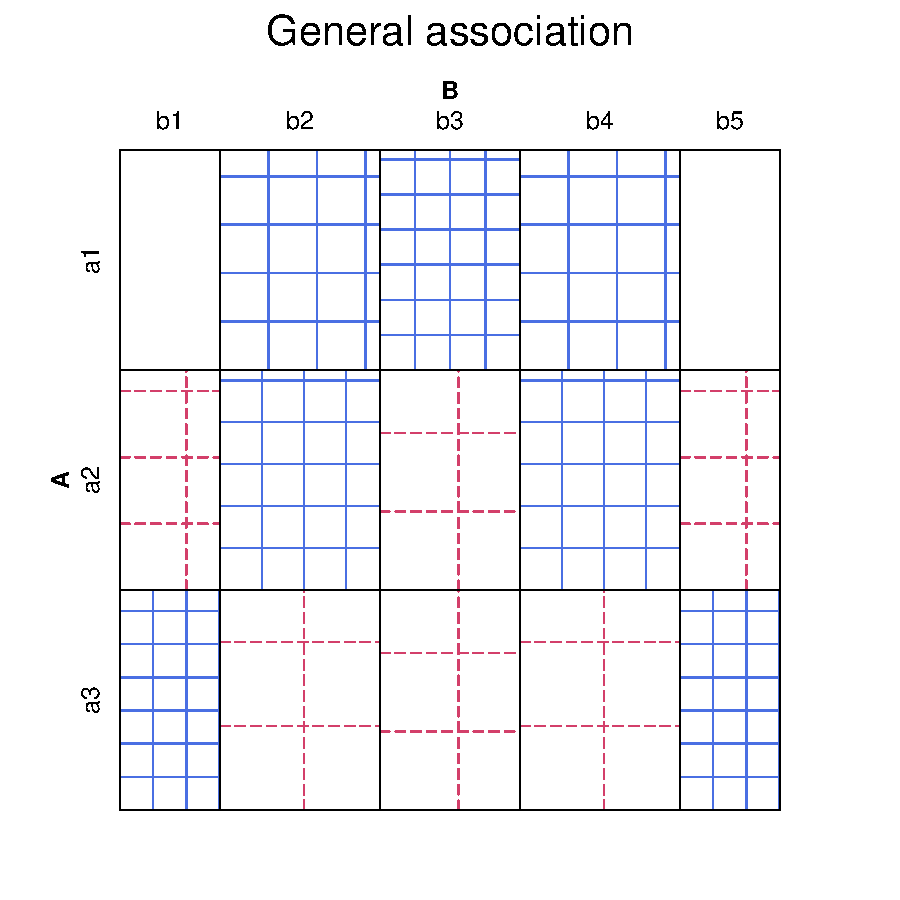
\includegraphics[width=.95\linewidth]{fig/cmhdemo1}
%  \caption{General association (sieve diagram)}\label{fig:cmhdemo1}
 \end{minipage}%
 \begin{minipage}[b]{.5\linewidth}
  \centering
  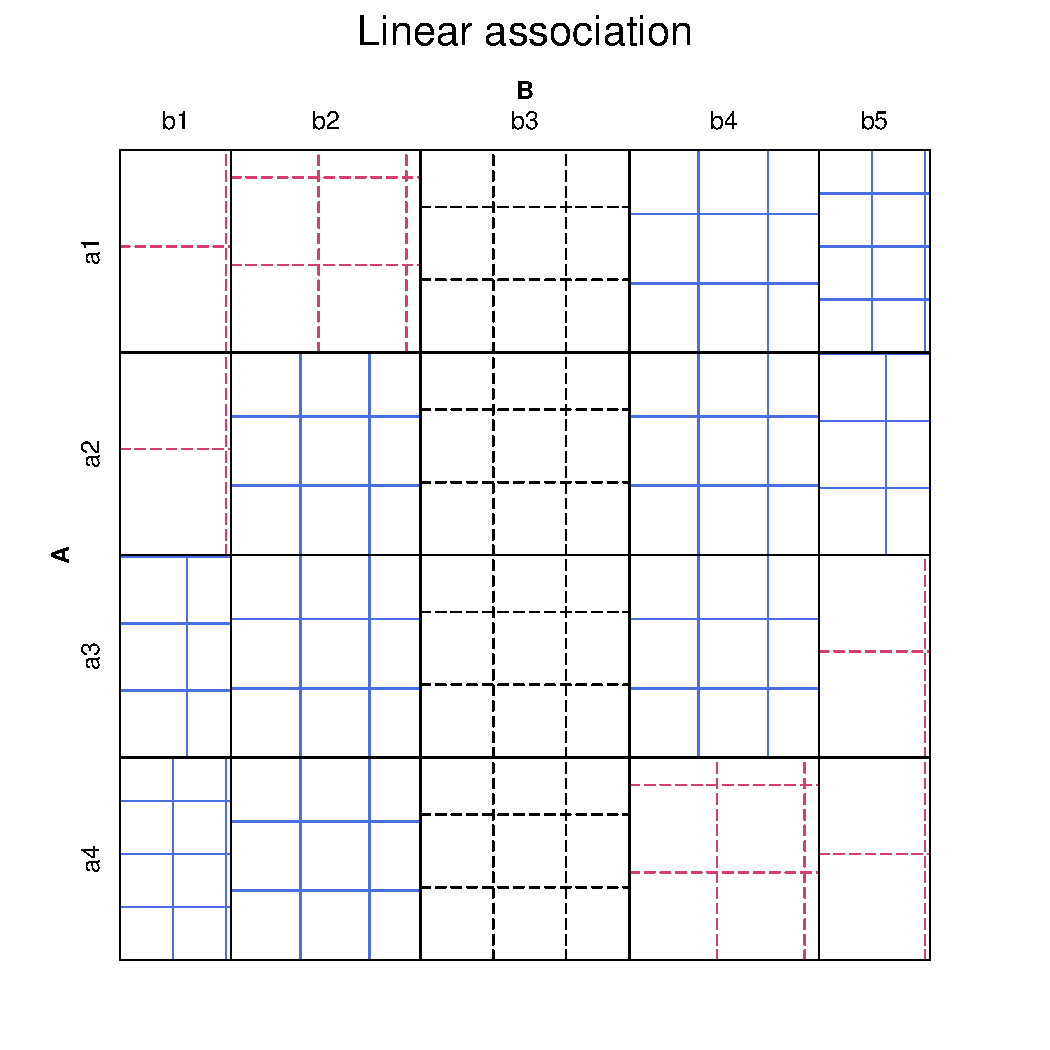
\includegraphics[width=.95\linewidth]{fig/cmhdemo2}
%  \caption{Linear association (sieve diagram)}\label{fig:cmhdemo2}
 \end{minipage}
\end{frame}

\subsection{Stratified analysis}
\begin{frame}[fragile]
  \frametitle{Stratified analysis}
  \begin{block}{\large\bfseries Overall analysis}
      \begin{itemize*}
	  \item ignores other variables (like sex), by collapsing over them
	  \item risks losing important interactions (e.g., different associations for M \& F)
	  \end{itemize*}
  \end{block}
  \begin{block}{\large\bfseries Stratified analysis}
      \begin{itemize*}
	  \item controls for the effects of one or more background variables
	  \item list stratification variable(s) \emph{first} on the \texttt{TABLES} statement
\begin{listing}[frame=single]
proc freq;
   tables \sasemph{age * sex} * treat * improve;
\end{listing}
	  \end{itemize*}
  \end{block}
  \begin{block}{Looking forward: Loglinear models}
      \begin{itemize*}
	  \item allow more general hypotheses to be stated and tested
	  \item closer connection between testing and visualization (\alert{how} are variables associated)
 	  \end{itemize*}
 \end{block}
\end{frame}

\begin{frame}[fragile]
  \frametitle{Stratified analysis}
The statements below request a stratified analysis with CMH tests,
controlling for sex.

\begin{Input}[fontsize=\footnotesize,label=\fbox{$\cdots$ \texttt{arthfreq.sas} $\cdots$},baselinestretch=0.8,firstnumber=20]
\sascomment{*-- Stratified analysis, controlling for sex;}
proc freq order=data;
   weight count;
   tables sex * treat * improve / cmh chisq nocol nopercent;
   run;
\end{Input}
$\rightarrow$ separate tables (partial tests) for Females and Males
\begin{Output}
       STATISTICS FOR TABLE 1 OF TREAT BY IMPROVE
               CONTROLLING FOR SEX=Female

 Statistic                     DF     Value        Prob
 ------------------------------------------------------
 Chi-Square                     2    11.296       0.004
 Likelihood Ratio Chi-Square    2    11.731       0.003
 Mantel-Haenszel Chi-Square     1    10.935       0.001
  ...
\end{Output}
\begin{itemize*}
\item Strong association between TREAT and IMPROVE for females
\end{itemize*}
\end{frame}

\begin{frame}[fragile]
Males:
\begin{Output}
       STATISTICS FOR TABLE 2 OF TREAT BY IMPROVE
                CONTROLLING FOR SEX=Male

 Statistic                     DF     Value        Prob
 ------------------------------------------------------
 Chi-Square                     2     4.907       0.086
 Likelihood Ratio Chi-Square    2     5.855       0.054
 Mantel-Haenszel Chi-Square     1     3.713       0.054
  ...

\sasemph{WARNING}:  67% of the cells have expected counts less
           than 5. Chi-Square may not be a valid test.
\end{Output}
\begin{itemize*}
\item Weak association between TREAT and IMPROVE for males
\item Sample size $N=29$ for males is small
\end{itemize*}

\end{frame}

\begin{frame}[fragile]
\frametitle{Stratified tests}
  \begin{itemize*}
    \item Individual (\emph{partial}) tests are followed by a \emph{conditional} test,
	controlling for strata (SEX)
	\item These tests {\bf do not} require large sample size in the individual
strata--- just a large total sample size.
    \item They \emph{assume}, but do not \emph{test} that the association is the
	same for all strata.
  \end{itemize*}

\begin{Output}[gobble=6]
                 SUMMARY STATISTICS FOR TREAT BY IMPROVE
                           CONTROLLING FOR SEX

        Cochran-Mantel-Haenszel Statistics (Based on Table Scores)

      Statistic   Alternative Hypothesis    DF       Value      Prob
      --------------------------------------------------------------
         1        Nonzero Correlation        1      14.632     0.000
         2        Row Mean Scores Differ     1      14.632     0.000
         3        General Association        2      14.632     0.001
\end{Output}

\end{frame}

\subsection{Homogeneity of association}
\begin{frame}[fragile]
  \frametitle{Homogeneity of association}
  \begin{itemize}
	\item Is the association between the primary table variables the same over all strata?
	\item 2 $\times$ 2 tables: $\rightarrow$ Equal odds ratios across all strata?
      \begin{itemize*}
	  \item \PROC{FREQ}: \texttt{MEASURES} option on \texttt{TABLES} statement $\rightarrow$ Breslow-Day test
\begin{listing}[frame=single]
 proc freq;
    tables strata * factor * response / \sasemph{measures cmh} ;
\end{listing}

	  \end{itemize*}
	\item Larger tables: Use \PROC{CATMOD} to test for \emph{no three-way association} 
       \begin{itemize*} 
        \item $\equiv$ \alert{same} association for the primary factor \& response variables $\forall$ strata
        \item $\equiv$\loglin\ model: [Strata Factor] [Strata Response] [Factor Response]
\begin{listing}[frame=single]
 proc catmod;
    ...
    loglin strata | factor | response @2;
\end{listing}
       \end{itemize*}
  \end{itemize}
\end{frame}

\begin{frame}[fragile]
  \frametitle{Homogeneity of association: Example}
  \begin{itemize}
	\item Arthritis data: homogeneity $\leftrightarrow$ no 3-way sex * treatment * outcome association
      \begin{itemize*}
	  \item $\equiv$ \loglin\ model: [SexTreat] [SexOutcome] [TreatOutcome] 
	  \item $\equiv$ \texttt{loglin sex|treat|improve@2} for \PROC{CATMOD}
	  \item Zero frequencies: \PROC{CATMOD} treats as ``structural zeros'' by default; recode if necessary.
	  \end{itemize*}
  \end{itemize}

\begin{Input}[fontsize=\footnotesize,label=\fbox{$\cdots$ \texttt{arthfreq.sas}},baselinestretch=0.8,firstnumber=26]
title2 'Test homogeneity of treat*improve association';
data arth;
   set arth;
   if count=0 then count=1E-20;   \sascomment{*-- sampling zeros;}
proc catmod order=data;
   weight count;
   model sex * treat * improve = _response_ / ml ;
   loglin \sasemph{sex|treat|improve @2} / title='No 3-way association';
run;
   loglin sex treat|improve   / title='No Sex Associations';
\end{Input}
\end{frame}

\begin{frame}[fragile]
  \frametitle{Homogeneity of association: Example}
  \begin{itemize*}
  \item the likelihood ratio \(\chi^2\) (the
badness-of-fit for the No 3-Way model) is the test for homogeneity
  \item clearly non-significant $\rightarrow$
treatment-outcome association can be considered to be the same for
men and women.
  \end{itemize*}
\begin{Output}[baselinestretch=0.75]
      Test homogeneity of treat*improve association
                   No 3-way association
      MAXIMUM-LIKELIHOOD ANALYSIS-OF-VARIANCE TABLE

    Source                   DF   Chi-Square      Prob
    --------------------------------------------------
    SEX                       1        14.13    0.0002
    TREAT                     1         1.32    0.2512
    SEX*TREAT                 1         2.93    0.0871
    IMPROVE                   2        13.61    0.0011
    SEX*IMPROVE               2         6.51    0.0386
    TREAT*IMPROVE             2        13.36    0.0013

    \sasemph{LIKELIHOOD RATIO}          2         1.70    \sasemph{0.4267}
\end{Output}
  \begin{itemize*}
  \item But, associations of \texttt{SEX*TREAT} and \texttt{SEX*IMPROVE}
  are both small.
  \item Suggests stronger model of homogeneity, [Sex] [TreatOutcome],
  tested by \texttt{loglin sex treat|improve;} statement.
  \end{itemize*}

\end{frame}

\begin{frame}[fragile]
  \frametitle{Homogeneity of association: Reduced model}
\begin{Input}[fontsize=\footnotesize,label=\fbox{$\cdots$ \texttt{arthfreq.sas}},baselinestretch=0.8,firstnumber=30]
proc catmod order=data;
   weight count;
   model sex * treat * improve = _response_ / ml ;
   loglin sex|treat|improve@2 / title='No 3-way association';
run;
   loglin \sasemph{sex treat|improve}   / title='No Sex Associations';
\end{Input}
Output:
\begin{Output}[baselinestretch=0.75]
                   No Sex Associations
      MAXIMUM-LIKELIHOOD ANALYSIS-OF-VARIANCE TABLE

    Source                   DF   Chi-Square      Prob
    --------------------------------------------------
    SEX                       1        12.95    0.0003
    TREAT                     1         0.15    0.6991
    IMPROVE                   2        10.99    0.0041
    TREAT*IMPROVE             2        12.00    0.0025

    LIKELIHOOD RATIO          5         9.81    \sasemph{0.0809}
\end{Output}
  \begin{itemize*}
  \item Fits reasonably well
  \item How to interpret?
  \end{itemize*}

\end{frame}

\begin{frame}
  \frametitle{Homogeneity of association}
\boldital{Visualizing Association:} Mosaic displays

\vspace{2ex}
 \begin{minipage}[b]{.5\linewidth}
  \centering
  \includegraphics[width=.95\linewidth,clip]{fig/arthmos1} \\ Baseline model
 \end{minipage}%
 \begin{minipage}[b]{.5\linewidth}
  \centering
  \includegraphics[width=.95\linewidth,clip]{fig/arthmos2}  \\ Reduced model
 \end{minipage}

\end{frame}

\endinput

% slide template
\begin{frame}
  \frametitle{}
  \begin{itemize}
	\item{\large\bfseries }
      \begin{itemize*}
	  \item 
    	\begin{itemize*}
		\item 
		\item 
		\end{itemize*}
	  \item 
	  \end{itemize*}
	\item{\large\bfseries }
	\item{\large\bfseries }
  \end{itemize}
\end{frame}

